\label{chap.7}

\section{Introduction and Prognostic Motivation}

The safe and economical deployment of lithium-ion battery packs
in safety-critical applications---such as aerospace vehicles,
electric powertrains, and grid storage---demands accurate state
of health (SOH) monitoring and remaining useful life (RUL) prognostics
\cite{saxena2015remaining, ge2021multistep}. In conventional battery
management literature, end-of-life (EOL) is almost universally defined as
the point at which cell discharge capacity drops below 80\% of its
rated initial capacity ($\mathrm{SOH} \le 0.80$)
\cite{bloom2001accelerated, han2019review}. Under this standard
paradigm, prognostic models track the monotonic decrease of capacity
over repeated duty cycles and extrapolate the trajectory forward in time
to predict the remaining ampere-hour throughput or cycle count
\cite{yang2018fast}.

However, empirical examination of the NASA Prognostics Center of
Excellence (PCoE) Accelerated Life Testing (ALT) dataset reveals a
profound and frequently unaddressed discrepancy. Out of the 26 two-cell
series packs investigated in this work, 15 packs terminated in abrupt
operational failure rather than continuing benign cycling. Crucially,
\textbf{10 of these 15 failure events occurred while the pack's
capacity was still strictly above 0.80 SOH}. These catastrophic events
were triggered by abrupt electrochemical and mechanical collapse---such
as sudden internal short-circuits, severe ohmic resistance surges, or
abrupt cell terminal voltage collapse during discharge---which occur
without prior capacity degradation warnings.

This finding carries vital engineering implications:
\begin{enumerate}
  \item A prognostic system relying exclusively on capacity fade cannot
  provide early warnings for the majority of field failure modes observed
  under high-stress or accelerated operating regimes.
  \item Health-conscious fast-charging algorithms that throttle current
  solely as a function of capacity loss may remain vulnerable to abrupt
  thermal and electrical breakdowns.
  \item Robust battery lifecycle assessment requires a dual-track
  prognostic framework that combines non-parametric survival analysis
  (capturing both gradual degradation and sudden failure) with
  predictive remaining useful life regression.
\end{enumerate}

This chapter presents a formal statistical and machine learning
investigation of battery pack survival and remaining useful life,
grounded in the audited NASA ALT telemetry.

\section{Cohort Stratification and Dataset Endpoints}

\subsection{Two-Cohort Stratification}

Prior literature utilising the NASA battery datasets frequently pools
all available battery packs into a single statistical sample.
However, the data audit performed in Chapter~\ref{chap.3} identified
substantial anomalies in the initial baseline capacities of three packs:
\texttt{battery13}, \texttt{battery36}, and \texttt{battery54}.
As documented in Table~\ref{tab:cohort_summary}, these three packs
exhibited initial reference discharge capacities below \SI{2.0}{Ah}
(specifically \SI{1.88}{Ah}, \SI{1.85}{Ah}, and \SI{1.87}{Ah},
respectively), compared to the nominal \SI{2.45}{Ah} exhibited by fresh
Samsung INR18650-25R cells.

\begin{table}[htbp]
  \centering
  \caption{Cohort stratification of the 26 NASA ALT battery packs.}
  \label{tab:cohort_summary}
  \resizebox{\columnwidth}{!}{%
  \begin{tabular}{lccl}
    \toprule
    \textbf{Cohort} & \textbf{Count} & \textbf{Initial Capacity (Ah)} & \textbf{Handling in Analysis} \\
    \midrule
    Original Main Cohort & 23 & $2.43 \pm 0.04$ & Primary statistical and survival sample \\
    Recommissioned Cohort & 3 & $< 2.00$ & Evaluated separately; excluded from main SOH EOL \\
    \bottomrule
  \end{tabular}%
  }
\end{table}

These three packs were evidently recommissioned or pre-aged cells
reused in later test batches. Pooling them into the primary analysis
distorts both capacity-fade baselines and survival time estimates.
Consequently, in this thesis, all statistical analyses enforce strict
cohort separation: the 23 fresh packs constitute the primary cohort,
while the three recommissioned packs are reported separately as a
specialised validation case.

\subsection{Failure Mode Classification and Census}

Script \texttt{24\_pack\_endpoints.py} conducted an exhaustive
end-of-telemetry audit across all 26 packs. Each pack was classified
into one of five mutually exclusive terminal states based on terminal
voltage stability, charge integrity, and reference capacity:
\begin{itemize}
  \item \textbf{event\_strong}: Verified hard electrochemical failure.
  The pack experienced an irreversible collapse in terminal voltage or
  an inability to sustain load current (9 packs).
  \item \textbf{event\_probable}: Probable pack failure or protection
  circuit trip. Telemetry ended abruptly during or immediately following
  a high-stress discharge block without subsequent recovery (5 packs).
  \item \textbf{event\_charger\_dead}: Catastrophic equipment failure
  or terminal disconnect. Observed in \texttt{battery23}, where the last
  charge block recorded an unphysical terminal voltage of
  $V_c = -0.111\,\mathrm{V}$ (1 pack).
  \item \textbf{transient\_collapse}: Temporary voltage instability
  followed by anomalous recovery. Observed in \texttt{battery54}, which
  experienced an isolated discharge collapse but subsequently recovered
  normal voltage profiles before test termination (1 pack, treated as censored).
  \item \textbf{no\_failure\_evidence}: Right-censored survivors. Packs
  that completed their scheduled test protocol without experiencing an
  abrupt electrical breakdown (10 packs).
\end{itemize}

\subsection{Sensitivity to SOH Normalisation Basis}

State of Health is defined as the ratio of current discharge capacity
to a reference capacity:
\begin{equation}
  \mathrm{SOH}_{\mathrm{abs}} = \frac{Q_{\mathrm{measured}}}{Q_{\mathrm{nom}}},
  \qquad
  \mathrm{SOH}_{\mathrm{rel}} = \frac{Q_{\mathrm{measured}}}{Q_0},
\end{equation}
where $Q_{\mathrm{nom}} = \SI{2.45}{Ah}$ is the nominal cell rating and
$Q_0$ is the specific pack's pristine initial capacity at cycle~0.

Table~\ref{tab:basis_sensitivity} details the outcome of evaluating the
classical $\mathrm{SOH} \le 0.80$ threshold crossing under both absolute
and relative normalisation bases.

\begin{table}[htbp]
  \centering
  \caption{Impact of SOH normalisation basis on EOL threshold crossings
  and failure precedence (Script \texttt{24\_pack\_endpoints.py}).}
  \label{tab:basis_sensitivity}
  \resizebox{\columnwidth}{!}{%
  \begin{tabular}{lcccc}
    \toprule
    \textbf{Cohort} & \textbf{Basis} & \textbf{Packs ($N$)} &
    \textbf{SOH $\le 0.80$ Crossers} & \textbf{Failures Before SOH Threshold} \\
    \midrule
    \multirow{2}{*}{Original Cohort} & Absolute & 23 & 12 & 8 of 13 failures \\
                                     & Relative & 23 & 11 & 11 of 13 failures \\
    \midrule
    \multirow{2}{*}{Recommissioned}  & Absolute & 3  & 3  & 0 of 2 failures \\
                                     & Relative & 3  & 0  & 2 of 2 failures \\
    \midrule
    \multirow{2}{*}{\textbf{Total Combined}} & Absolute & 26 & 15 & \textbf{8 of 15 failures} \\
                                             & Relative & 26 & 11 & \textbf{13 of 15 failures} \\
    \bottomrule
  \end{tabular}%
  }
\end{table}

Under the relative SOH basis, \textbf{13 out of 15 failures (86.7\%)}
occurred before the cell reached the 80\% capacity retention limit.
Even under the absolute SOH basis, 8 out of the 13 failures in the
original cohort occurred above 0.80 SOH. Figure~\ref{fig:soh_distribution}
illustrates the distribution of SOH at the final recorded reference check.
Packs such as \texttt{battery21} and \texttt{battery30} suffered fatal
breakdowns at absolute SOH values of 0.908 and 0.889, respectively,
corresponding to less than 10\% capacity degradation.

\begin{figure}[htbp]
  \centering
  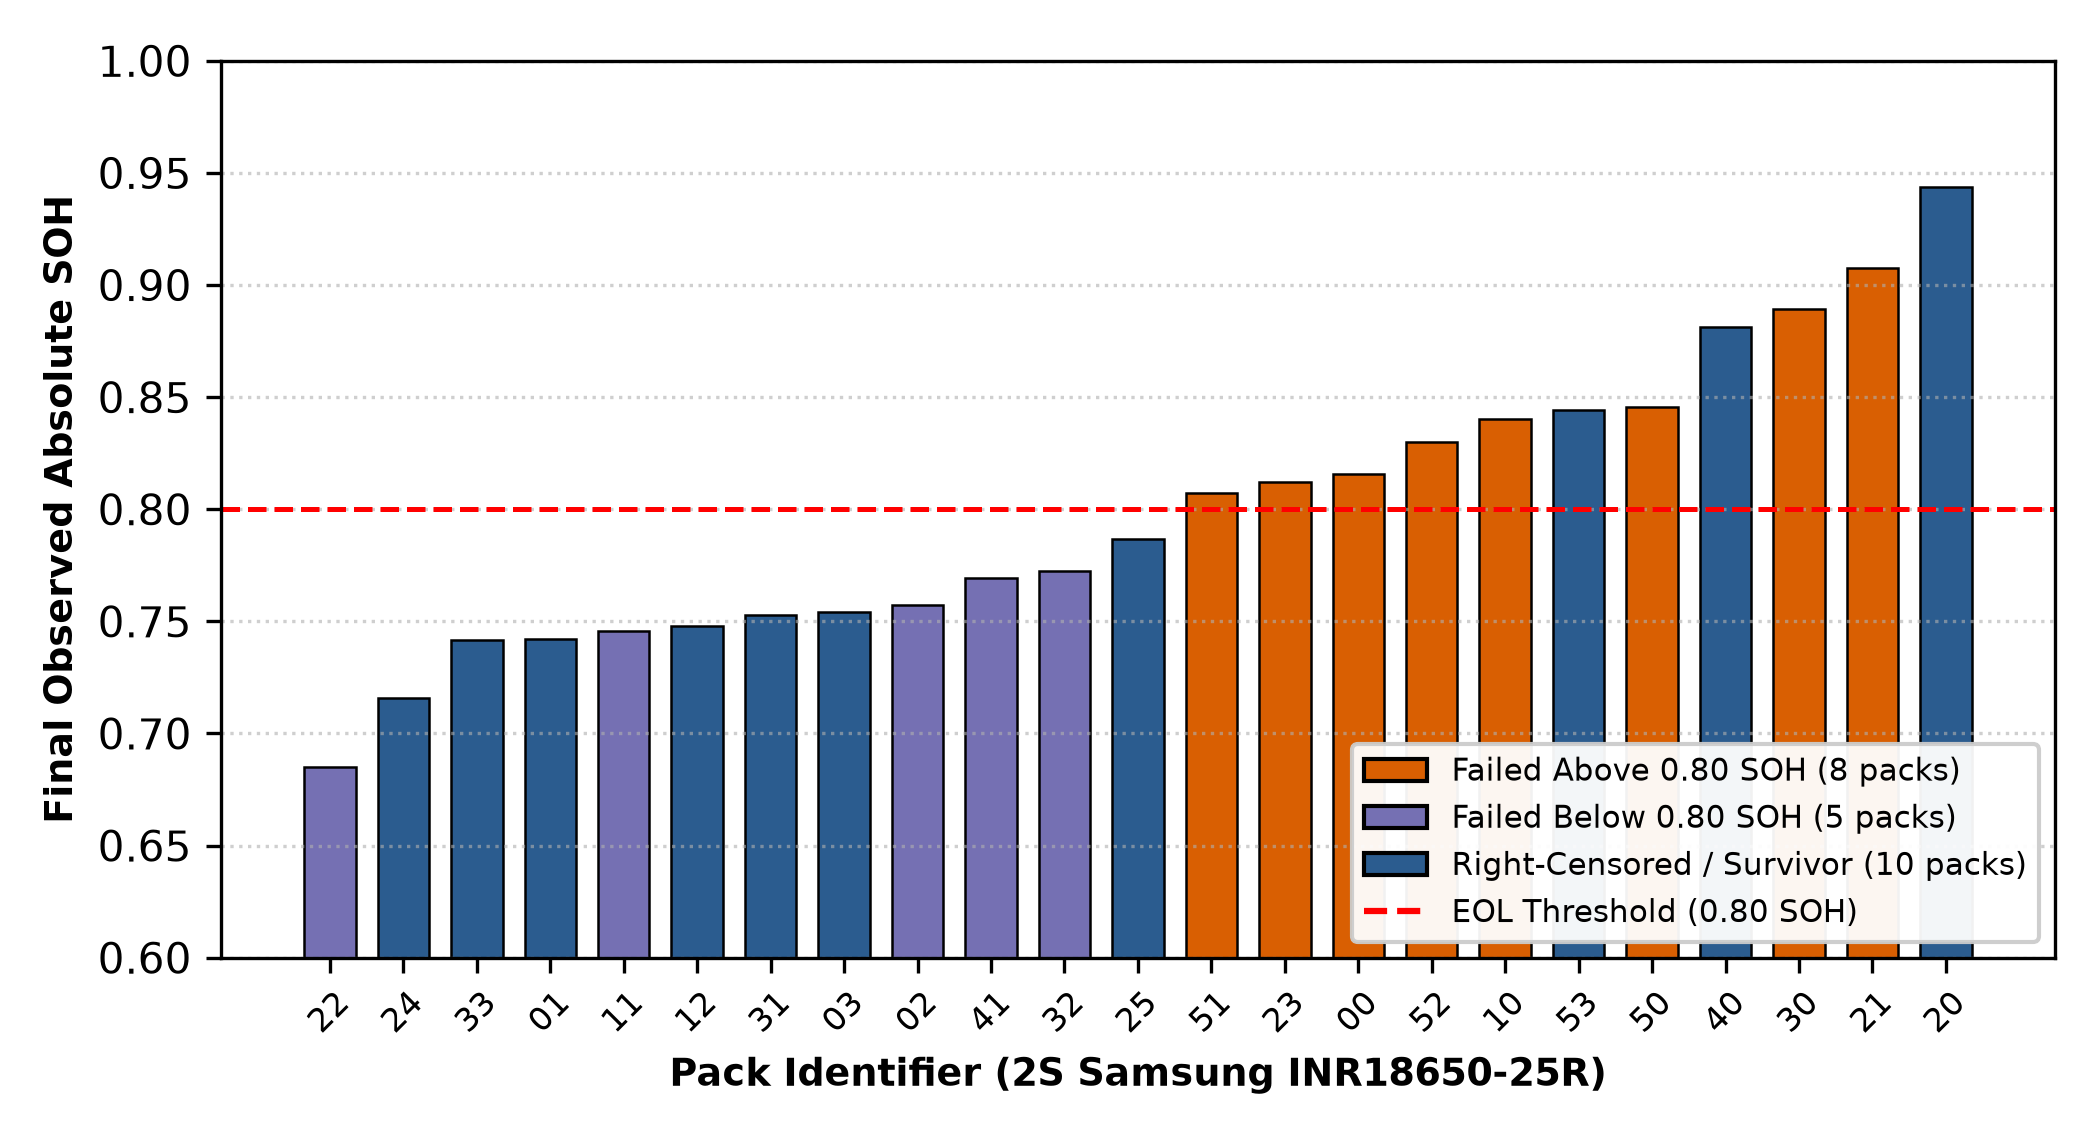
\includegraphics[width=0.88\textwidth]{soh_distribution.png}
  \caption[Final recorded State of Health across primary cohort]{Final recorded State of Health ($\mathrm{SOH}_{\mathrm{abs}}$) across
  all 23 packs of the primary cohort. Over half of the failing packs (8 of 13)
  experienced terminal operational breakdown while capacity remained strictly
  above the classical 0.80 EOL threshold (red dashed line).}
  \label{fig:soh_distribution}
\end{figure}

\section{Kaplan--Meier Nonparametric Survival Analysis}

\subsection{Mathematical Formulation}

To model pack lifetime without imposing unverified parametric assumptions
(e.g., Weibull or exponential distributions), we formulate an
interval-censored survival model using the product-limit estimator of
Kaplan and Meier \cite{kaplan1958nonparametric}.

Let $T$ denote the total cumulative discharge throughput (in ampere-hours,
$\mathrm{Ah}$) until an endpoint event. For a set of ordered distinct event
throughputs $t_1 < t_2 < \dots < t_k$, the estimated survival probability
$\hat{S}(t) = P(T > t)$ is defined by:
\begin{equation}
  \hat{S}(t) = \prod_{i:\, t_i \le t} \left( 1 - \frac{d_i}{n_i} \right),
  \label{eq:kaplan_meier}
\end{equation}
where $d_i$ represents the number of observed failure events at throughput
$t_i$, and $n_i$ is the number of packs remaining at risk immediately prior
to $t_i$ (i.e., packs that have neither experienced an event nor been censored
prior to $t_i$).

Because reference capacity checks were conducted intermittently (nominally
after every 20 mission cycles), the exact moment of threshold crossing
lies within an inspection interval $[t_{\mathrm{prev}}, t_{\mathrm{obs}}]$.
To maintain conservative bounds, failure events that occurred during mission
cycles following the final reference check are interval-censored over
$[t_{\mathrm{last\_ref}},\, t_{\mathrm{last\_ref}} + \SI{60}{Ah}]$.

\subsection{Three Distinct Operational Endpoint Formulations}

To separate capacity exhaustion from functional breakdown, we define
three alternative endpoint criteria:
\begin{itemize}
  \item \textbf{Endpoint A (SOH $\le 0.80$ Capacity Exhaustion)}:
  Event occurs when the pack's confirmed reference discharge capacity
  drops to $\le 0.80 \cdot Q_{\mathrm{nom}}$. Packs that fail abruptly
  prior to crossing 0.80 are treated as right-censored at their final
  recorded throughput.
  \item \textbf{Endpoint B (Composite Retirement)}:
  Event occurs at the earliest occurrence of either: (i) capacity dropping
  below 0.80 SOH, or (ii) abrupt operational pack failure. This represents
  the true real-world service lifetime of the pack.
  \item \textbf{Endpoint C (Abrupt Functional Breakdown)}:
  Event occurs strictly upon physical or electrical failure
  (\texttt{event\_strong}, \texttt{event\_probable}, or
  \allowbreak\texttt{event\_charger\_dead}). Packs that reach 0.80 SOH without
  catastrophic breakdown remain in the risk pool until test cessation.
\end{itemize}

\subsection{Empirical Survival Curves and Median Lifetimes}

Script \texttt{25\_survival\_rul.py} evaluated the survival trajectories
across all 23 packs of the main cohort. The resulting survival functions
are plotted in Figure~\ref{fig:km_curves}, and the key survival statistics
are summarised in Table~\ref{tab:km_results}.

\begin{figure}[htbp]
  \centering
  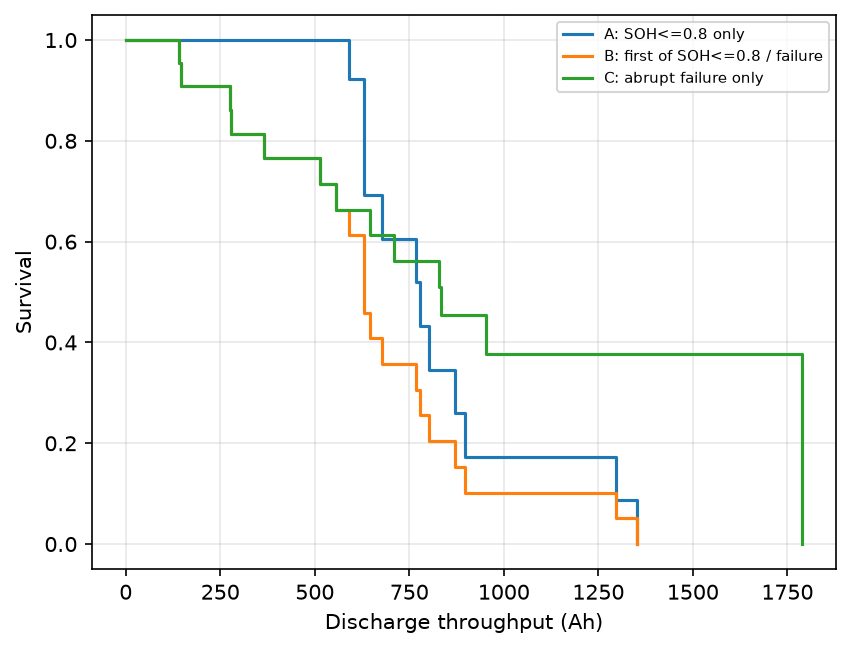
\includegraphics[width=0.82\textwidth]{km_v73.png}
  \caption[Kaplan--Meier survival curves across three operational endpoints]{Kaplan--Meier survival curves for the primary NASA ALT cohort
  ($N = 23$) across three distinct operational endpoint definitions:
  Endpoint~A (capacity fade only), Endpoint~B (first of capacity fade or
  abrupt failure), and Endpoint~C (abrupt functional failure only).}
  \label{fig:km_curves}
\end{figure}

\begin{table}[htbp]
  \centering
  \caption{Kaplan--Meier survival statistics across the three endpoint
  definitions for the primary cohort ($N = 23$).}
  \label{tab:km_results}
  \resizebox{\columnwidth}{!}{%
  \begin{tabular}{lccc}
    \toprule
    \textbf{Endpoint Definition} & \textbf{Observed Events} &
    \textbf{Censored Packs} & \textbf{Median Throughput (Ah)} \\
    \midrule
    \textbf{Endpoint A}: SOH $\le 0.80$ only & 12 / 23 & 11 / 23 & \SI{777.7}{Ah} \\
    \textbf{Endpoint B}: First of SOH $\le 0.80$ or failure & \textbf{20 / 23} & 3 / 23 & \textbf{630.5}{Ah} \\
    \textbf{Endpoint C}: Abrupt failure only & 13 / 23 & 10 / 23 & \SI{833.2}{Ah} \\
    \bottomrule
  \end{tabular}%
  }
\end{table}

The survival analysis demonstrates a stark quantitative reality:
\begin{enumerate}
  \item Under Endpoint~A (the standard capacity-fade benchmark), the
  estimated median lifetime is \textbf{\SI{777.7}{Ah}}. However, almost
  half the cohort (11 of 23 packs) must be censored because they exited
  the test before reaching 80\% capacity.
  \item Under Endpoint~B (composite operational retirement), the median
  throughput drops sharply to \textbf{\SI{630.5}{Ah}}, representing a
  \textbf{18.9\% reduction in expected operational life}. Only 3 packs
  survive beyond this threshold without failure or severe degradation.
  \item Under Endpoint~C, catastrophic electrical failures exhibit a median
  survival throughput of \textbf{\SI{833.2}{Ah}}. The earliest sudden
  failures appear as early as \SI{141.8}{Ah} (\texttt{battery30}) and
  \SI{146.2}{Ah} (\texttt{battery21}), demonstrating that abrupt failure
  is not restricted to highly aged cells.
\end{enumerate}

\section{Remaining Useful Life Prediction via LOPO Regression}

\subsection{Problem Formulation and Dataset Filtering}

For battery packs undergoing gradual degradation, the Remaining Useful Life
(RUL) at cumulative throughput $t$ is defined as the additional throughput
$\Delta t_{\mathrm{rem}}$ required to reach the EOL threshold
$t_{\mathrm{cross}}$:
\begin{equation}
  \mathrm{RUL}(t) = \max\left(0,\, t_{\mathrm{cross}} - t\right).
\end{equation}

To construct a rigorous prognostic benchmark that avoids data leakage,
we apply two structural constraints:
\begin{enumerate}
  \item \textbf{Trajectory Depth Filtering}: Packs with 7 or fewer reference
  checks (Packs 10, 20, 21, 30, 40, and 50) lack
  sufficient historical baseline points to establish reliable degradation
  derivatives and are excluded from the regression set.
  \item \textbf{Leave-One-Pack-Out (LOPO) Cross-Validation}: To guarantee
  unseen generalisation, evaluation is performed across 12 eligible
  threshold-crossing packs comprising 193 individual reference check
  observations. In each LOPO fold, all observations from pack $p$ are held
  out entirely, while the model is trained exclusively on the remaining
  11 packs.
\end{enumerate}

\subsection{Feature Engineering}

At each reference inspection cycle $k$, the feature vector
$\mathbf{x}_k \in \mathbb{R}^3$ comprises:
\begin{equation}
  \mathbf{x}_k = \begin{bmatrix}
    \mathrm{Throughput}_k \\
    \mathrm{SOH}_{\mathrm{abs}, k} \\
    \Delta\mathrm{SOH}_{100, k}
  \end{bmatrix},
\end{equation}
where $\Delta\mathrm{SOH}_{100, k}$ is the local capacity degradation rate
computed over a three-reference lookback window, normalised to capacity
lost per \SI{100}{Ah} of throughput:
\begin{equation}
  \Delta\mathrm{SOH}_{100, k} = \frac{\mathrm{SOH}_k - \mathrm{SOH}_{k-3}}
  {t_k - t_{k-3}} \times 100.
\end{equation}

\subsection{Benchmark Models}

We benchmark three predictive paradigms:
\begin{enumerate}
  \item \textbf{Population Median Baseline (\texttt{pop})}:
  Predicts remaining life based on the training cohort's median crossing
  throughput:
  \begin{equation}
    \widehat{\mathrm{RUL}}_{\mathrm{pop}}(t) = \max\left(0,\,
    \mathrm{Median}\left(\{t_{\mathrm{cross}, j}\}_{j \ne p}\right) - t\right).
  \end{equation}

  \item \textbf{Deterministic Linear Extrapolation (\texttt{linear})}:
  Extrapolates the current capacity state to the 0.80 threshold using the
  instantaneous degradation slope:
  \begin{equation}
    \widehat{\mathrm{RUL}}_{\mathrm{linear}}(t) = \mathrm{clip}\left(
    \frac{\mathrm{SOH}_{\mathrm{abs}}(t) - 0.80}
    {-\Delta\mathrm{SOH}_{100}(t) / 100},\, 0,\, 2000 \right).
  \end{equation}

  \item \textbf{Standardised Ridge Regression (\texttt{ridge})}:
  Fits an L2-regularised linear model with penalty parameter $\alpha = 1.0$
  on z-score standardised features:
  \begin{equation}
    \min_{\mathbf{w}} \|\mathbf{y}_{\mathrm{train}} - \mathbf{Z}\mathbf{w}\|_2^2
    + \alpha \|\mathbf{w}\|_2^2,
    \qquad
    \mathbf{Z} = \frac{\mathbf{X}_{\mathrm{train}} - \boldsymbol{\mu}_{\mathbf{X}}}
    {\boldsymbol{\sigma}_{\mathbf{X}}}.
  \end{equation}
\end{enumerate}

\subsection{Empirical Prognostic Performance}

Table~\ref{tab:rul_performance} presents the cross-validated RUL prediction
metrics across all 193 test points and for the critical near-EOL regime
($\mathrm{RUL} \le \SI{200}{Ah}$).

\begin{table}[htbp]
  \centering
  \caption{Leave-One-Pack-Out (LOPO) RUL prediction performance over
  12 packs and 193 reference observations.}
  \label{tab:rul_performance}
  \resizebox{\columnwidth}{!}{%
  \begin{tabular}{lcccc}
    \toprule
    \textbf{Model} & \textbf{Overall MAE (Ah)} & \textbf{RMSE (Ah)} &
    $R^2$ \textbf{Score} & \textbf{Near-EOL MAE ($\le \SI{200}{Ah}$)} \\
    \midrule
    Population Median (\texttt{pop}) & 187.0 & 262.7 & 0.074 & \SI{96.5}{Ah} \\
    Linear Extrapolation (\texttt{linear}) & 133.9 & 207.8 & 0.421 & \textbf{\SI{46.6}{Ah}} \\
    \textbf{Ridge Regression (\texttt{ridge})} & \textbf{113.0} & \textbf{141.4} & \textbf{0.732} & \SI{58.8}{Ah} \\
    \bottomrule
  \end{tabular}%
  }
\end{table}

Ridge regression achieves the superior global performance, reducing overall
MAE to \textbf{\SI{113.0}{Ah}} (a 39.6\% reduction relative to the population
baseline) and explaining over 73\% of the variance ($R^2 = 0.732$).
The deterministic linear extrapolation model suffers from high variance
early in pack life due to small divisor noise in the slope estimate
($\mathrm{RMSE} = \SI{207.8}{Ah}$), but excels in the final \SI{200}{Ah}
prior to threshold crossing ($\mathrm{MAE} = \SI{46.6}{Ah}$), where local
fade rates stabilise.

Figure~\ref{fig:rul_parity} presents the Leave-One-Pack-Out parity plot
along with the prognostic uncertainty distribution across battery lifecycle stages.

\begin{figure}[htbp]
  \centering
  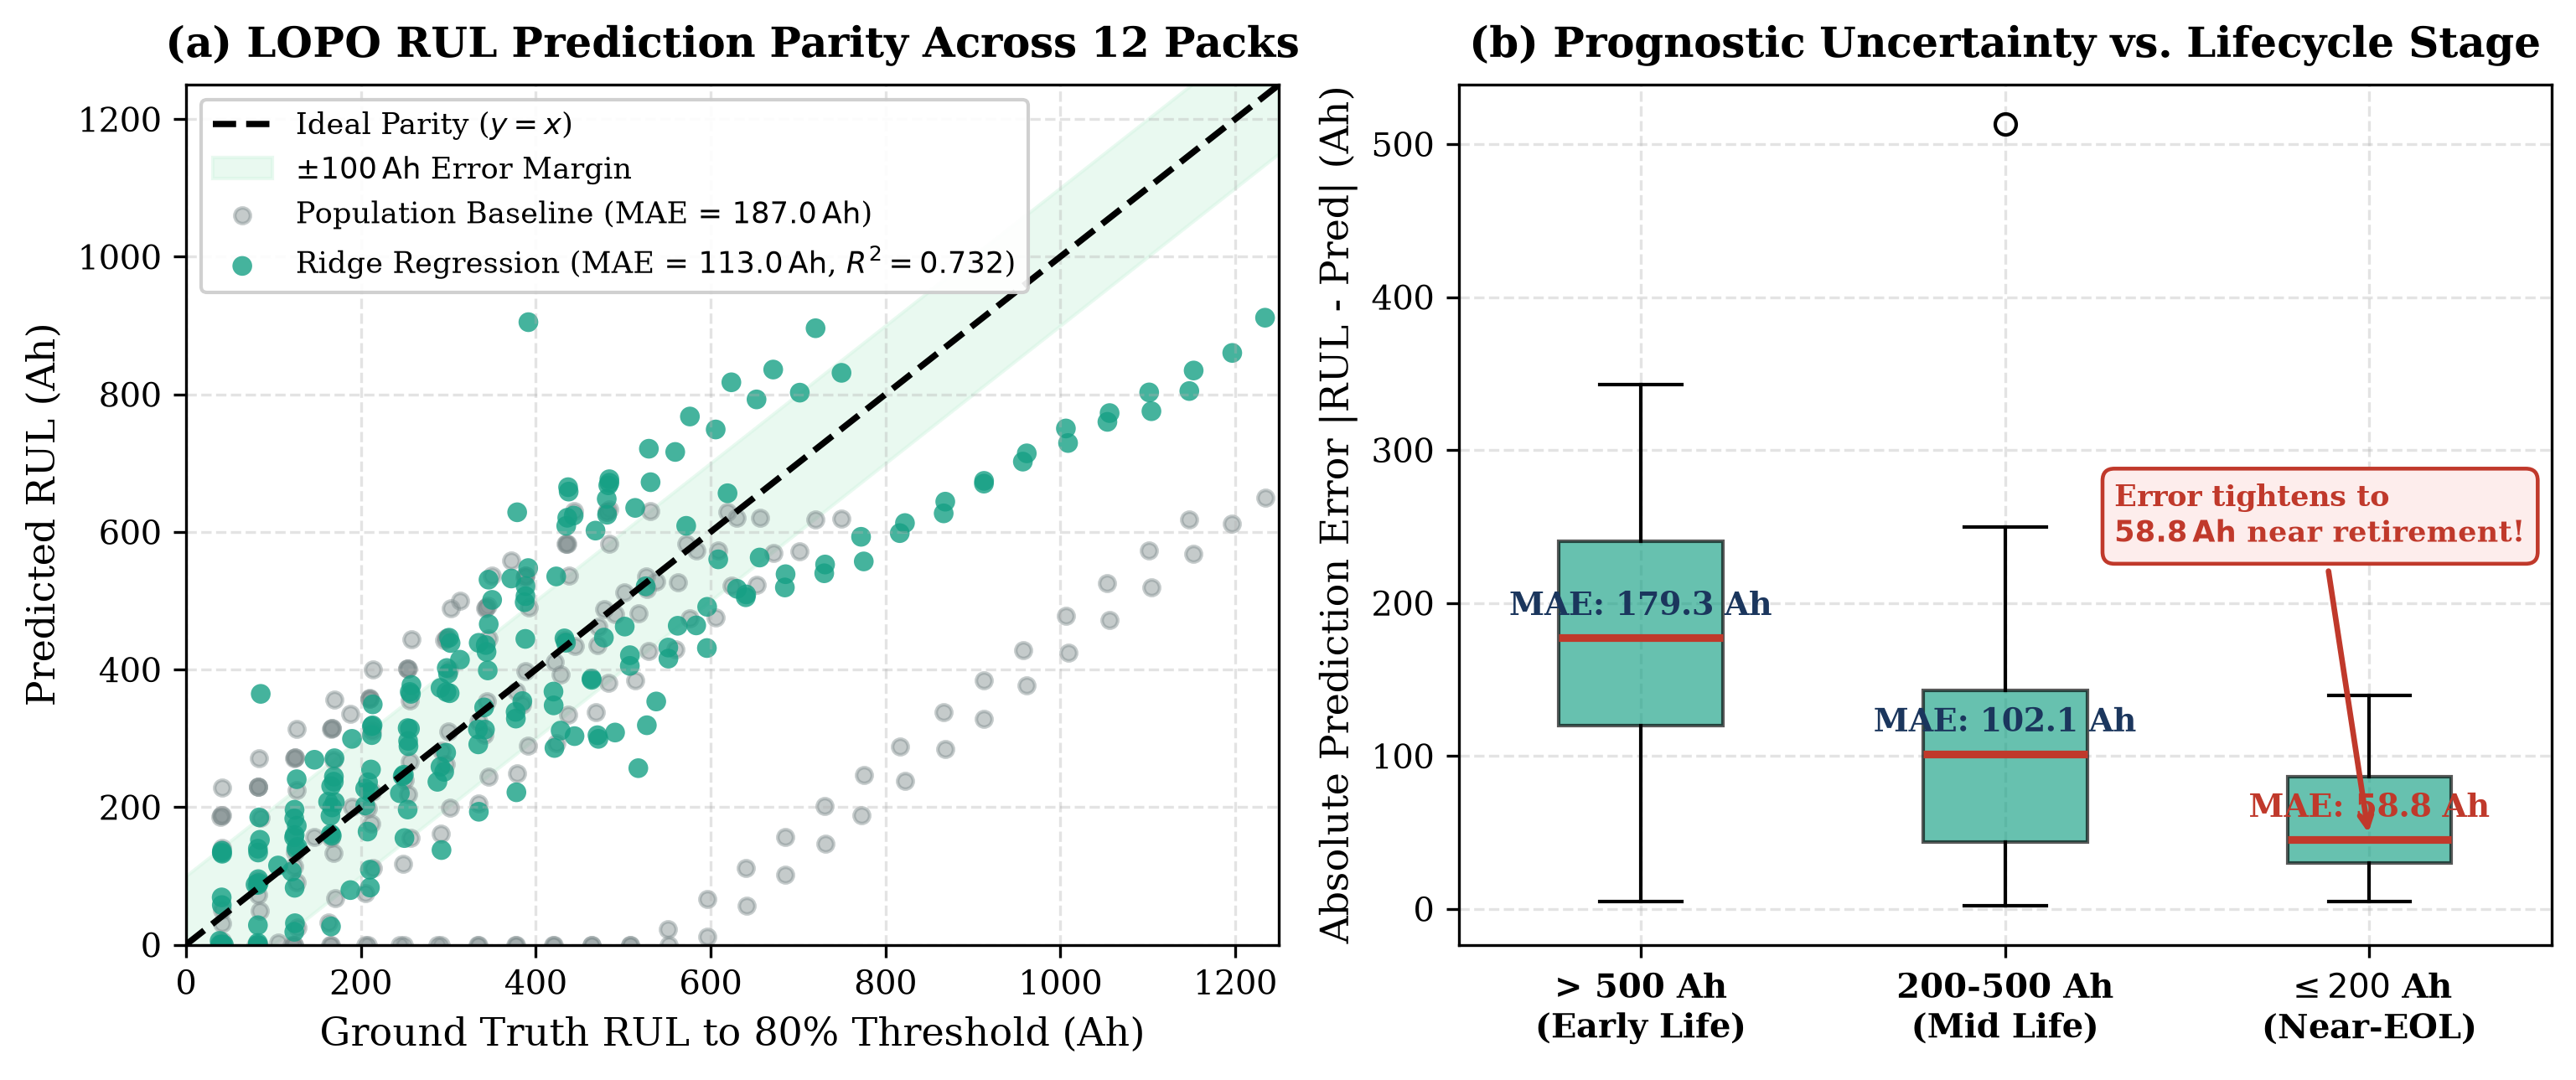
\includegraphics[width=0.95\textwidth]{ch7_rul_parity_plot.png}
  \caption[Leave-One-Pack-Out RUL prediction parity and uncertainty shrinkage]{Leave-One-Pack-Out (LOPO) Remaining Useful Life (RUL) prognostic
  performance across 12 threshold-crossing packs and 193 reference inspections.
  (a) Parity plot of predicted vs.\ ground-truth RUL (Ah), demonstrating strong
  linear correlation for regularised Ridge regression ($\mathrm{MAE} = 113.0\,\mathrm{Ah},
  R^2 = 0.732$) relative to the population median baseline ($\mathrm{MAE} = 187.0\,\mathrm{Ah}$).
  (b) Absolute prediction error distribution stratified by lifecycle stage,
  highlighting substantial prognostic uncertainty reduction to an MAE of
  $58.8\,\mathrm{Ah}$ as the battery approaches the critical $\le 200\,\mathrm{Ah}$
  near-EOL boundary.}
  \label{fig:rul_parity}
\end{figure}

Table~\ref{tab:per_pack_mae} itemises the individual pack-level error
breakdown for the Ridge model.

\begin{table}[htbp]
  \centering
  \caption{Per-pack Ridge regression MAE across the 12 evaluation packs.}
  \label{tab:per_pack_mae}
  \begin{tabular}{lc|lc}
    \toprule
    \textbf{Pack ID} & \textbf{Ridge MAE (Ah)} & \textbf{Pack ID} & \textbf{Ridge MAE (Ah)} \\
    \midrule
    \texttt{battery01} & 144.0 & \texttt{battery24} & 114.0 \\
    \texttt{battery02} &  71.0 & \texttt{battery25} &  74.0 \\
    \texttt{battery03} &  97.0 & \texttt{battery31} &  91.0 \\
    \texttt{battery11} & 154.0 & \texttt{battery32} &  79.0 \\
    \texttt{battery12} &  62.0 & \texttt{battery33} & 126.0 \\
    \texttt{battery22} & 117.0 & \texttt{battery41} & 163.0 \\
    \bottomrule
  \end{tabular}
\end{table}

The lowest prediction errors are achieved on packs exhibiting steady,
consistent wear (\texttt{battery12}: \SI{62.0}{Ah}; \texttt{battery02}:
\SI{71.0}{Ah}). The largest errors occur on \texttt{battery41}
(\SI{163.0}{Ah}), which experienced severe non-monotonic capacity
fluctuations, and \texttt{battery11} (\SI{154.0}{Ah}), which sustained
an exceptionally prolonged cycle life exceeding \SI{1700}{Ah} of throughput.

\section{Prognostic Integration with the MA-BMS Framework}

The findings of this chapter directly reshape the control architecture
developed in Chapter~\ref{chap.5}:

\begin{enumerate}
  \item \textbf{Reframing the Health-Cap Agent}: The health-cap controller
  was originally conceived to extend cycle life by throttling current to
  reduce capacity fade. However, since the majority of ALT failures occur
  at high SOH due to thermal and resistance overstress rather than capacity
  exhaustion, a static capacity-based health cap is misaligned with the
  dominant failure mechanisms.
  \item \textbf{Dynamic Resistance Monitoring}: The empirical evidence that
  sudden breakdowns are preceded by internal resistance divergence reinforces
  the critical necessity of the 4-state adaptive EKF. By tracking the ohmic
  scaling factor $\rho_k$ at every second, the safety supervisor protects
  the battery against sudden overvoltage even when capacity appears healthy.
  \item \textbf{Hybrid Prognostic Supervisor}: An operational BMS must
  integrate the continuous RUL estimate $\widehat{\mathrm{RUL}}(t)$ with the
  instantaneous voltage margin $\Delta V_{\mathrm{margin}}$. When
  $\widehat{\mathrm{RUL}}$ drops below a critical threshold or when
  $\hat{\rho}$ surges abruptly, the supervisory logic initiates
  preventative derating, converting sudden catastrophic collapse into a
  graceful operational shutdown.
\end{enumerate}
